\def\ktitle{ASSEMBLY ASSIGNMENT}
\def\kauthor{Koushik Kalyani}
\def\kcontact{koushikkalyani369@gmail.com}
\def\kmodule{IITH - Future Wireless Communication}
%\renewcommand{\thesection}{\arabic{section}}
%\renewcommand{\thesubsection}{\arabic{subsection}}
%\titleformat{\subsubsection}{\normalfont\itshape\filcenter}{\thesubsubsection}{1em}{}
\documentclass[journal,12pt,twocolumn]{IEEEtran}
\usepackage{enumitem}
%\renewcommand{\thesection}{\arabic{section}}
%\renewcommand{\thesubsection}{\arabic{subsection}}
\usepackage{tikz}
\usepackage{circuitikz}
\usepackage{karnaugh-map}
\usepackage{tabularx}
\usepackage{circuitikz}
\usepackage{tikz}
\usepackage{titlesec}
\usepackage{multirow}
\title{\ktitle}
\author{\kauthor\\\kcontact\\\kmodule}
\begin{document}
\maketitle
\tableofcontents
\section{\textbf{Question}}
 The digital circuit shown \rule{9mm}{0.4pt}
\begin{figure}[ht]
    \centering
    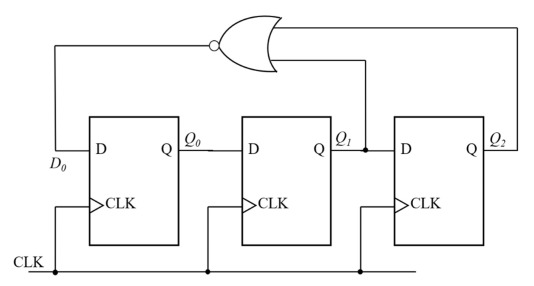
\includegraphics[width=0.45\columnwidth,height=0.45\columnwidth]{asmq.jpeg}
   % \caption{Caption}
    \label{fig:enter-label}
\end{figure}
\section{\textbf{Answer}}
The above question can be solved by using Truth Table and karnaugh-map.
\subsection{\centering Truth Table}
\begin{tabularx}{0.45\textwidth}{
 | >{\centering\arraybackslash}X
 | >{\centering\arraybackslash}X
 | >{\centering\arraybackslash}X
 | >{\centering\arraybackslash}X
 | >{\centering\arraybackslash}X
 | >{\centering\arraybackslash}X
        | >{\centering\arraybackslash}X
        | >{\centering\arraybackslash}X
        | >{\centering\arraybackslash}X|}
    \hline
  \multicolumn{3}{|c}{Present State} & \multicolumn{3}{|c}{Flip-Flop i/p} & \multicolumn{3}{|c|}{Next State}\\ 
    \hline
\textbf{$Q_0$}&\textbf{$Q_1$}&\textbf{$Q_2$}&\textbf{$D_0$}&\textbf{$D_1$}&\textbf{$D_2$}&\textbf{$Q_0'$}&\textbf{$Q_1'$}&\textbf{$ Q_2'$}\\
 \hline
 0&0&0&1&0&0&1&0&0\\
 \hline
 1&0&0&1&1&0&1&1&0\\
 \hline
        1&1&0&0&1&1&0&1&1\\
 \hline
 0&1&1&0&0&1&0&0&1\\
 \hline
 0&0&1&0&0&0&0&0&0\\
 \hline
 \end{tabularx}
\begin{figure}
\subsection{\centering K-Map Implentation}
\resizebox{0.45\textwidth}{!}{%
 \begin{karnaugh-map}[4][2][1][$Q_1Q_2$][$Q_0$]
  \maxterms{1,2,3,5,6,7}
  \minterms{4,0}
  \implicant{0}{4}
  %\implicant{4}{12}
  %\implicantedge{12}{12}{14}{14}
 \end{karnaugh-map}%
}
 \centering \textbf{ $D_0=\overline Q_1\cdot \overline Q_2$}
\resizebox{0.45\textwidth}{!}{%
 \begin{karnaugh-map}[4][2][1][$Q_1Q_2$][$Q_0$]
  \maxterms{1,2,3,5,0,7}
  \minterms{4,6}
  \implicantedge{4}{4}{6}{6}
  %\implicant{4}{12}
  %\implicantedge{12}{12}{14}{14}
 \end{karnaugh-map}%
}
\centering \textbf{ $D_1= Q_0\cdot \overline Q_2$}
\resizebox{0.45\textwidth}{!}{%
 \begin{karnaugh-map}[4][2][1][$Q_1Q_2$][$Q_0$]
  \maxterms{1,2,4,5,0,7}
  \minterms{3,6}
  \implicant{3}{3}
            \implicant{6}{6}
  %\implicant{4}{12}
  %\implicantedge{12}{12}{14}{14}
 \end{karnaugh-map}%
}
\centering \textbf{ $D_2= \overline Q_0\cdot Q_1\cdot Q_2 + Q_0\cdot Q_1 \cdot \overline Q_2$ }
\end{figure}
 \vspace{\baselineskip}
Therefore, given circuit is Divide by 5 circuit.
 \section{\textbf{Components}}
 \begin{tabularx}{0.45\textwidth}{
   | >{\centering\arraybackslash}X
   | >{\centering\arraybackslash}X
   | >{\centering\arraybackslash}X |
   }
   \hline
   \textbf{Components}&\textbf{Values}&\textbf{Quantity}\\
   \hline
   Arduino & Uno & 1\\
   \hline
   Jumper Wires & M-M & 25\\
   \hline
   Breadboard & & 1\\
   \hline
                LED & & 3\\
                \hline
                Resistor & $ \geq 220\Omega$&3\\
                \hline
                Flip Flop & 7474 & 2 \\
\hline  
 \end{tabularx}
\section{\textbf{Implementation}}
\begin{tabular}{|c|c|c|c|c|c|c|c|c|c|c|c|c|}      
\hline                              
\multirow{2}{*}{} & \multicolumn{3}{c|}{INPUT} & \multicolumn{3}{c|}{OUTPUT} & \multicolumn{2}{|c}{\multirow{2}{*}{CLOCK}} & \multicolumn{4}{|c|}{\multirow{3}{*}{5V}} \\      
\cline{2-7}     
& Q0 & Q1 & Q2 & Q0' & Q1' & Q2' & \multicolumn{2}{|c|}{\multirow{2}{*}{}} & \multicolumn{4}{|c|}{} \\        
\hline          
Arduino & D9 & D10 & D11 & D2 & D3 & D4 & \multicolumn{2}{|c|}{A5} &
\multicolumn{4}{|c|}{\multirow{3}{*}{}}\\                                   
\hline                             
7474 & 5 & 9 &  & 2 & 12 &  & CLK1 & CLK2 & 1 & 4 & 10 & 13 \\                   
\hline                     
7474 & & & 9 & & & 12 & CLK1 & CLK2 & 1 & 4  & 10 & 13 \\                       
\hline                         
             
\end{tabular}
\begin{center}
    Connections
\end{center}
\textbf{Procedure}
\begin{enumerate}[label={\arabic*}.]
 \item Connect the circuit as per the above table.
 \item Connect LEDs to the output pins of the Arduino to see output.
 \item Execute the circuit using the below code.
  \vspace{\baselineskip}\\
                \begin{tabularx}{0.45\textwidth}{
    | >{\centering\arraybackslash}X|}
   \hline
https://github.com/koushikkalyani/FWC/blob/\\main/Assembly/assembly.asm\\
   \hline
  \end{tabularx}\\
  \vspace{\baselineskip}
  \item Visit for video demonstration .
         \vspace{\baselineskip}\\
  \begin{tabularx}{0.45\textwidth}{| >{\centering\arraybackslash}X|}
   \hline
https://github.com/koushikkalyani/FWC/blob/\\main/Assembly/AssemblyDemo.mp4\\
   \hline
  \end{tabularx}
  \end{enumerate}
\end{document}
